\section{Spherical Geometry}
In this section, we present some definitions and results from spherical geometry in order to prove a result which we rely on crucially in the coming sections.  We seek to prove the following lemma:\\

\noindent\textbf{\Cref{lem:sphtri}.}
\emph{The sum of the interior angles of a spherical triangle is strictly greater than $\pi$.  More specifically, the sum of the interior angles is equal to $\pi$ plus the area of the triangle.}


Throughout, we work with respect to the \textit{unit sphere} embedded naturally in $\R^3$ as the set of points satisfying $x^2+y^2+z^2=1$.  This sphere has radius 1, and therefore surface area equal to $4\pi$.  All of the results here carry through for a sphere of any radius $r$, and the only adjustment to be made is to multiply all of the areas by $r^2$.  For the convenience of notation and exposition, we note that our sphere is centered at the point $(0,0,0)$.

First, we need to define the concept of a \textit{spherical line}.  


\begin{figure}[htb]
	\centering
	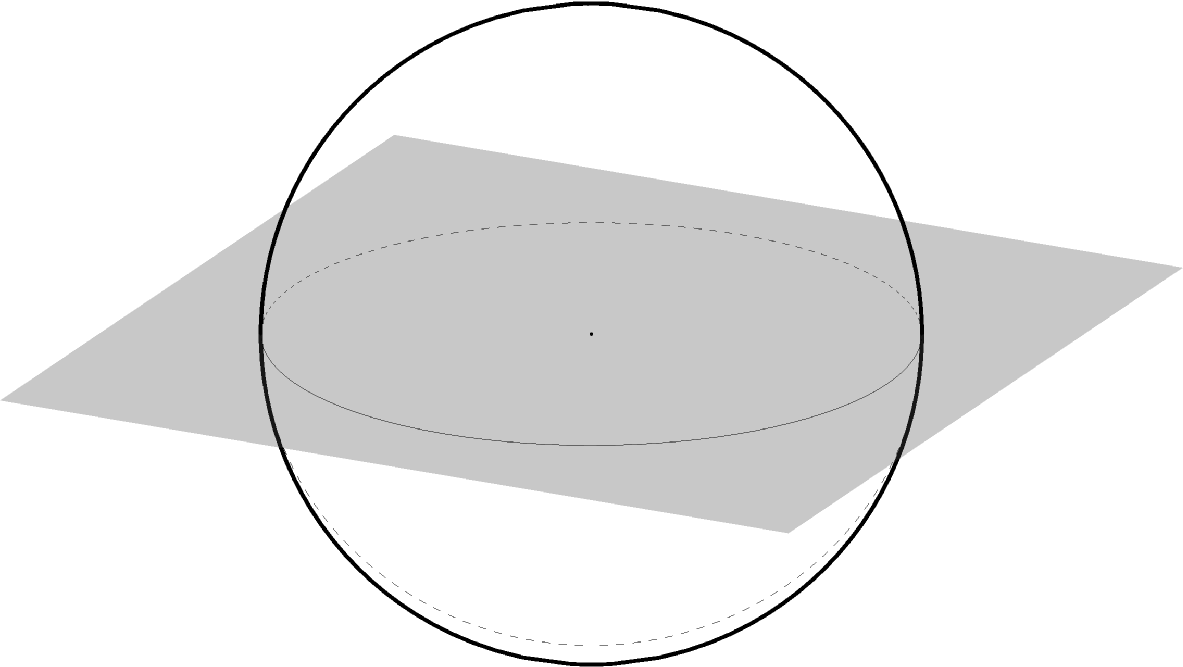
\includegraphics[width=.5\textwidth]{figs/sph-1pl.pdf}
	\caption{A great circle on the sphere with its identifying plane.}
	\label{fig:sphereline}
\end{figure}


\begin{definition}
On the sphere, the lines are \textit{great circles}, which are the circles of the largest possible radius on the surface of the sphere.  Equivalently, they are the intersections of the surface of the sphere with a plane passing through the center of the sphere.
\end{definition}  


Since spherical geometry can be hard to visualize, it helps to have an example in mind.  On the Earth, the lines of longitude are great circles, as is the equator.  Other latitudes are \textit{not} great circles.






We now present the observations which majorly differentiate spherical and planar geometry.

\begin{claim}
	Given any two points $p$ and $q$ on the sphere which are not antipodal (meaning that our points aren't of the form $p=(x,y,z)$ and $q=(-x,-y,-z)$), there is a unique great circle through $p$ and $q$. 
\end{claim}

To see this, consider the characterization of great circles as the intersections of the surface of the sphere with planes through the center of the sphere.  Since $p$ and $q$ are not antipodes, they are not both collinear with $(0,0,0)$ and so these three points uniquely determine a plane.  This plane intersects the sphere along a great circle which contains $p$ and $q$.

\begin{figure}[htb]
	\centering
	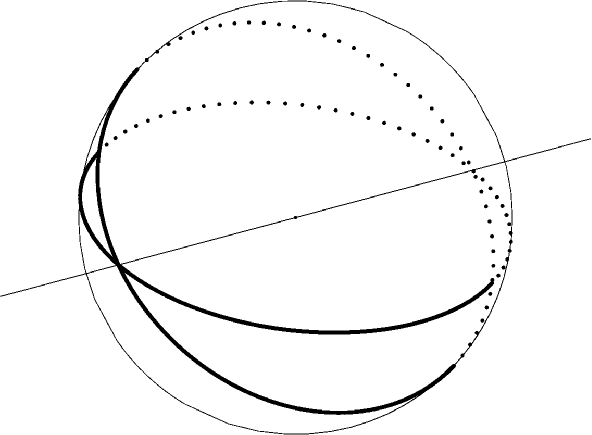
\includegraphics[width=.35\textwidth]{figs/2gc.pdf}
	\caption{Two great circles meet at antipodal points.}
	\label{fig:2gc}
\end{figure}


\begin{claim}
	Any pair of distinct great circles on the sphere intersect exactly twice, and the points of intersection are antipodes.
\end{claim}

Any two distinct planes determine two distinct great circles, and these planes intersect along a line in $\R^3$ which passes through $(0,0,0)$ and therefore meets the sphere itself at exactly two points, which must be antipodes.

Why is this weird? In the plane, it's the case that any pair of distinct lines intersects exactly once or they never intersect, in which case we call them \textit{parallel}. Since distinct great circles on the sphere intersect exactly twice, there is no such thing as `parallel lines' on the sphere, and we have to be careful about discussing `the' intersection of two great circles since they do not meet at a unique point.  Furthermore, it is not the case that there is a unique segment of a great circle connecting any two points; there are two, but unless these two points are antipodes, one of the two segments will be shorter.  As a convention, when we discuss `the' segment connecting two points, we mean the shorter one.  As an example, the shortest path from the North Pole of the Earth to London is to travel south along the $0^\circ$ line of longitude, not to travel along the $180^\circ$ line of longitude to the South Pole and then north along the $0^\circ$ line back up to London.

We now have enough machinery to sensibly define a \textit{spherical triangle} and observe some of its properties. Given three points $a$, $b$, and $c$ on the sphere, we can look at the shortest great circle segments connecting each pair of points.  This cuts the sphere into two regions, one with area at most $\pi$ and one with area at least $3\pi$.  The triangle is smaller of these two regions.


Unlike in the plane, the sum of the interior angles of a spherical triangle is not always a constant like $\pi$.  On the Earth if we take our three points to be the North Pole, the point at zero longitude and latitude (off the southern coast of Ghana), and the point at $90^\circ E$ longitude and zero latitude (a few hundred miles west of Indonesia), we get a triangle with three right angles, for a total measure of $\tfrac{3\pi}{2}$.



In order to  show \Cref{lem:sphtri}, we need some way to translate between \textit{angles} and \textit{area}.  To do that, we'll use a shape which doesn't even exist in the plane: the \textit{diangle} or \textit{lune}.  Consider two distinct great circles.  We know they intersect at two antipodal points, and we can also see that they cut the surface of the sphere into four regions.  Consider one of these regions.  Its boundary is a pair of great circle segments which connect antipodal points, and meet at some angle $\theta$ at both of these points, so this shape is like a polygon with two sides, hence the name `diangle'.  The name `lune' refers to the crescent moon-shape of this kind of region, and is the term we will use going forward.  On the Earth, a lune is the region between any two lines of longitude, for example.

The area of a lune with angle $\theta$ is easy to compute.


\begin{figure}[htb]
	\centering
	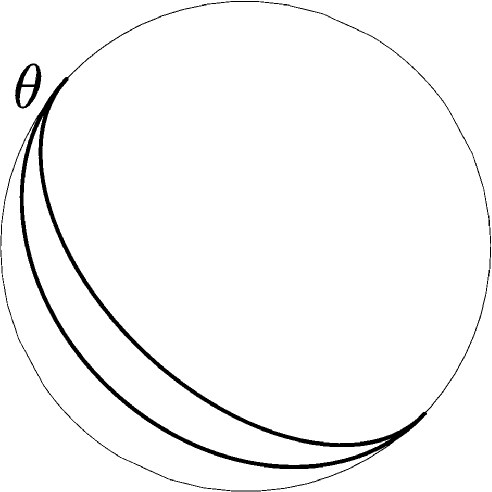
\includegraphics[width=.35\textwidth]{figs/lune.pdf}
	\caption{A lune corresponding to an angle $\theta$. }
	\label{fig:lune}
\end{figure}

\begin{claim}
	Consider a lune whose boundary segments meet at angle $\theta$.  Then the area of this lune is $2\theta$.
\end{claim}

This claim follows from observing that a lune with angle $\theta$ occupies a $\tfrac{2\pi}{\theta}$ portion of the sphere's surface area.  The total surface area of the sphere is $4\pi$, so a lune with angle $\theta$ has surface area $\tfrac{4\pi\theta}{2\pi}= 2\theta$.


Now that we have a tool that lets us relate angles and areas, we can finally prove the main result of this section.






	



\begin{lemma}\label{lem:sphtri}
	
The sum of the interior angles of a spherical triangle is strictly greater than $\pi$.  More specifically, the sum of the interior angles is equal to $\pi$ plus the area of the triangle.
\end{lemma}

\begin{proof}
	Consider a triangle on the sphere with angles $\theta_1$, $\theta_2$, and $\theta_3$.  Let $T$ denote the area of this triangle. If we extend the sides of the triangle to their entire great circles, each pair intersects at the vertices of our triangle as well as the three points antipodal to the vertices of our triangle, and at the same angles at both sets of points.  This triangle is congruent to our triangle, so its area is also $T$.  Each pair of lines cuts the sphere into four lunes, one which contains our triangle, one which contains the antipodal triangle, and two which do not contain either triangle.  We are interested in the three pairs of lunes which do contain the triangles.  We will label these lunes by their angles, so we have a lune $L(\theta_1)$ and its antipodal lune $L'(\theta_1)$, and we can similarly define $L(\theta_2)$, $L'(\theta_2)$, $L(\theta_3)$, and $L'(\theta_3)$.
	
	
	\begin{figure}[htb]
		\centering
		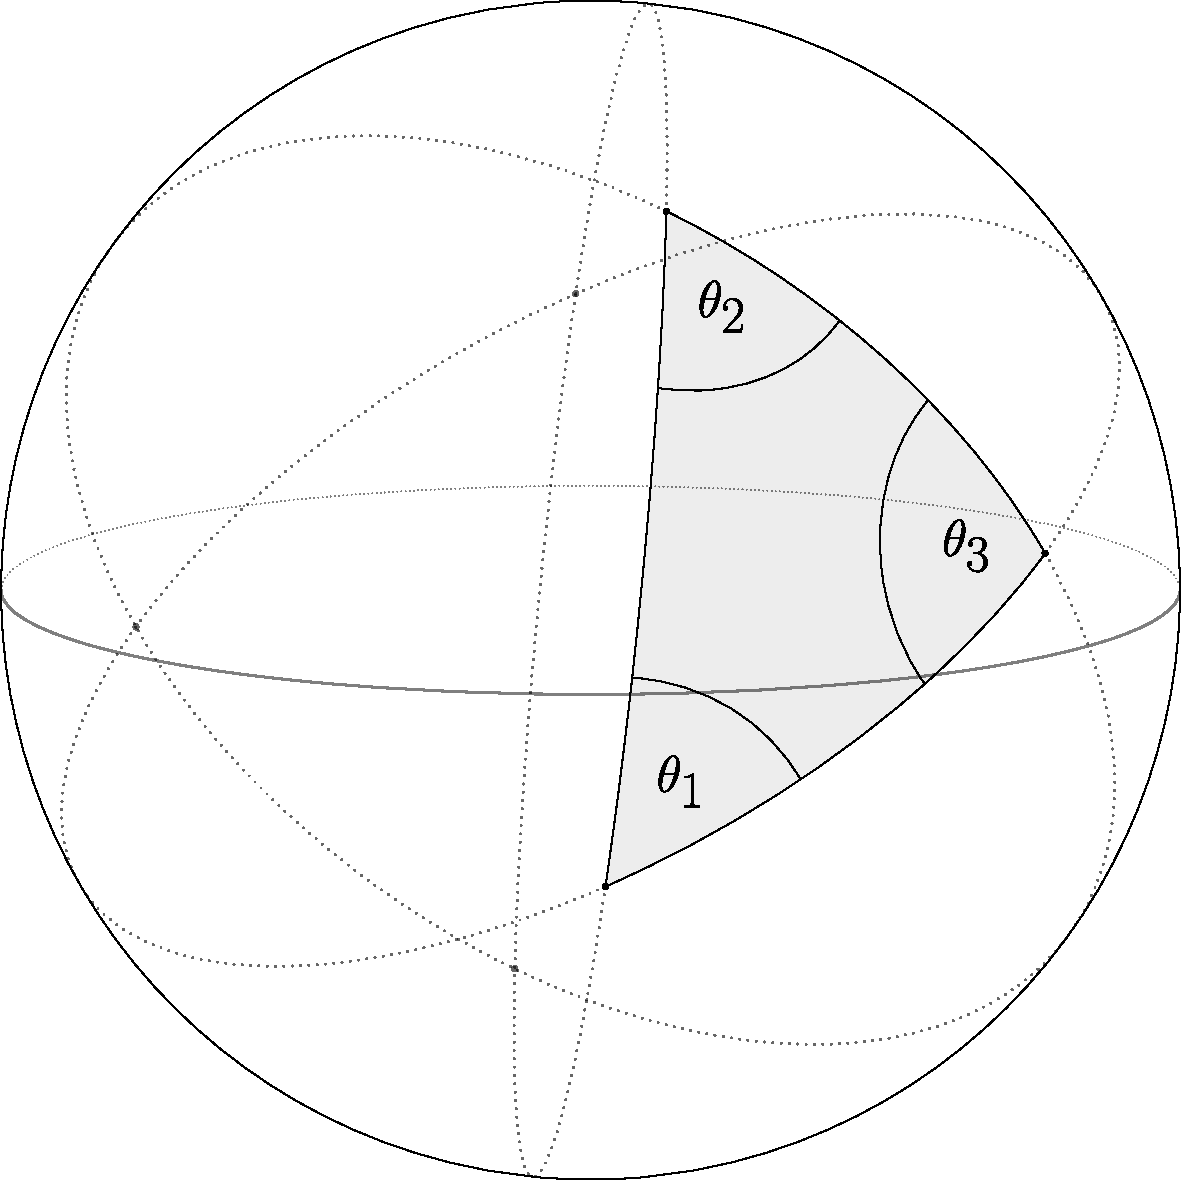
\includegraphics[width=.35\textwidth]{figs/trilune.pdf}
		\caption{A spherical triangle and the antipodal triangle define six lunes.}
		\label{fig:trilune}
	\end{figure}
	
	
	We have six lunes.  In total, they cover the sphere, but they do overlap.  If we remove our triangle from two of the three which contain it and the antipodal triangle from two of the three which contain it, then we have six non-overlapping regions which cover the sphere, so the area of the sphere must be equal to the sum of the areas of these six regions.  We can write
	
	\begin{align*}
	4\pi &= \mathrm{area}(L(\theta_1)) + \mathrm{area}(L'(\theta_1)) \\
	&+  (\mathrm{area}(L(\theta_2)) - T) + (\mathrm{area}(L'(\theta_2)) - T) \\
	&+ (\mathrm{area}(L(\theta_3)) - T)	 + (\mathrm{area}(L'(\theta_3)) - T).
	\end{align*}
	
And by the earlier claim, we know that the areas of the lunes are twice their angles, so we can rewrite this as


	\begin{align*}
4\pi &= 2\theta_1 + 2\theta_1 
+  (2\theta_2 - T) + (2\theta_2-T) 
+ (2\theta_3 - T)	 + (2\theta_3 - T)
\end{align*}

which simplifies to 

	\begin{align*}
\theta_1+\theta_2+\theta_3 = \pi + T.
\end{align*}

\end{proof}

We will need one more fact about spherical triangles before we conclude this section.  We do not prove it, but it dates back to (at least) Euclid's \textit{Elements} \cite{elements} where it follows from Propositions I.6 and I.8.  

\begin{fact}
	An equilateral triangle is equiangular, and vice versa.
\end{fact}

While \textit{Elements} is a compendium of facts about planar geometry, these two propositions do not rely on the assumption that parallel lines exist, and so they hold on the surface of the sphere as well.  To show them, first suppose that we have a triangle with vertices $a$, $b$, and $c$ and suppose that the length of the side $ab$ is equal to that of $bc$, and let $m$ be the midpoint of the segment $bc$.  Consider the segment $am$. This splits the triangle $abc$ into two triangles $amb$ and $amc$ which have equal side lengths and are therefore congruent.  By this congruence, the angle opposite $a$ is equal to the angle opposite $c$.

To see the converse, suppose that the angles opposite $a$ and $c$ are equal.  Then the triangles $abc$ and $acb$ are congruent, since \Cref{lem:sphtri} implies that if there are two triangles with the same angles, then their areas are equal as well and they are therefore congruent.

\zs{probably want to say something to wrap up here}

